\documentclass[14pt]{beamer}
\usepackage[T2A]{fontenc}
\usepackage[utf8]{inputenc}
\usepackage[english,russian]{babel}
\usepackage{amssymb,amsfonts,amsmath,mathtext}
\usepackage{cite,enumerate,float,indentfirst}

\graphicspath{{../images/}{images/}} 

\usepackage{../Dissertation/phdstyle}
\usepackage[edges]{forest}
%\newcommand{\W}{\Omega}
\newcommand{\Wedm}{\W^{edm}}
\newcommand{\Wmdm}{\W^{mdm}}
\newcommand{\gef}{\gamma_{eff}}

\usepackage{animate}
\usepackage{tcolorbox}

% \usetheme[secheader]{Boadilla}
% \usecolortheme{seahorse}

%\usetheme{Pittsburgh}
%\usecolortheme{whale}

\usetheme{Boadilla}

\beamertemplatenavigationsymbolsempty

\newcommand{\todo}{\alert}
%%% Основные сведения %%%
\newcommand{\thesisAuthorLastName}{\todo{Аксентьев}}
\newcommand{\thesisAuthorOtherNames}{\todo{Александр Евгеньевич}}
\newcommand{\thesisAuthorInitials}{\todo{А.\,Е.}}
\newcommand{\thesisAuthor}             % Диссертация, ФИО автора
{%
    \texorpdfstring{% \texorpdfstring takes two arguments and uses the first for (La)TeX and the second for pdf
        \thesisAuthorLastName~\thesisAuthorOtherNames% так будет отображаться на титульном листе или в тексте, где будет использоваться переменная
    }{%
        \thesisAuthorLastName, \thesisAuthorOtherNames% эта запись для свойств pdf-файла. В таком виде, если pdf будет обработан программами для сбора библиографических сведений, будет правильно представлена фамилия.
    }
}
\newcommand{\thesisAuthorShort}        % Диссертация, ФИО автора инициалами
{\thesisAuthorInitials~\thesisAuthorLastName}
%\newcommand{\thesisUdk}                % Диссертация, УДК
%{\todo{xxx.xxx}}
\newcommand{\thesisTitle}              % Диссертация, название
{\todo{Метод замороженного спина  для поиска электрического дипольного момента дейтрона в накопительном кольце}}
\newcommand{\thesisSpecialtyNumber}    % Диссертация, специальность, номер
{\todo{01.04.01}}
\newcommand{\thesisSpecialtyTitle}     % Диссертация, специальность, название
{\todo{Приборы и методы экспериментальной физики}}
\newcommand{\thesisDegree}             % Диссертация, ученая степень
{\todo{кандидата физико-математических наук}}
\newcommand{\thesisDegreeShort}        % Диссертация, ученая степень, краткая запись
{\todo{канд. физ.-мат. наук}}
\newcommand{\thesisCity}               % Диссертация, город написания диссертации
{\todo{Москва}}
\newcommand{\thesisYear}               % Диссертация, год написания диссертации
{\todo{2019}}
\newcommand{\thesisOrganization}       % Диссертация, организация
{\todo{Национальный Ядерный Исследовательский Университет ``МИФИ'' \\ (НИЯУ МИФИ)}}
\newcommand{\thesisOrganizationShort}  % Диссертация, краткое название организации для доклада
{\todo{НазУчДисРаб}}

\newcommand{\thesisInOrganization}     % Диссертация, организация в предложном падеже: Работа выполнена в ...
{\todo{учреждении, в~котором выполнялась данная диссертационная работа}}

\newcommand{\supervisorFio}            % Научный руководитель, ФИО
{\todo{Сеничев Юрий Валериевич}}
\newcommand{\supervisorRegalia}        % Научный руководитель, регалии
{\todo{д.ф.-.м.н., проф.}}
\newcommand{\supervisorFioShort}       % Научный руководитель, ФИО
{\todo{Ю.\,В.~Сеничев}}
\newcommand{\supervisorRegaliaShort}   % Научный руководитель, регалии
{\todo{уч.~ст.,~уч.~зв.}}


\newcommand{\opponentOneFio}           % Оппонент 1, ФИО
{\todo{Фамилия Имя Отчество}}
\newcommand{\opponentOneRegalia}       % Оппонент 1, регалии
{\todo{доктор физико-математических наук, профессор}}
\newcommand{\opponentOneJobPlace}      % Оппонент 1, место работы
{\todo{Не очень длинное название для места работы}}
\newcommand{\opponentOneJobPost}       % Оппонент 1, должность
{\todo{старший научный сотрудник}}

\newcommand{\opponentTwoFio}           % Оппонент 2, ФИО
{\todo{Фамилия Имя Отчество}}
\newcommand{\opponentTwoRegalia}       % Оппонент 2, регалии
{\todo{кандидат физико-математических наук}}
\newcommand{\opponentTwoJobPlace}      % Оппонент 2, место работы
{\todo{Основное место работы c длинным длинным длинным длинным названием}}
\newcommand{\opponentTwoJobPost}       % Оппонент 2, должность
{\todo{старший научный сотрудник}}

\newcommand{\leadingOrganizationTitle} % Ведущая организация, дополнительные строки
{\todo{Федеральное государственное бюджетное образовательное учреждение высшего профессионального образования с~длинным длинным длинным длинным названием}}

\newcommand{\defenseDate}              % Защита, дата
{\todo{DD mmmmmmmm YYYY~г.~в~XX часов}}
\newcommand{\defenseCouncilNumber}     % Защита, номер диссертационного совета
{\todo{Д\,123.456.78}}
\newcommand{\defenseCouncilTitle}      % Защита, учреждение диссертационного совета
{\todo{Название учреждения}}
\newcommand{\defenseCouncilAddress}    % Защита, адрес учреждение диссертационного совета
{\todo{Адрес}}
\newcommand{\defenseCouncilPhone}      % Телефон для справок
{\todo{+7~(0000)~00-00-00}}

\newcommand{\defenseSecretaryFio}      % Секретарь диссертационного совета, ФИО
{\todo{Фамилия Имя Отчество}}
\newcommand{\defenseSecretaryRegalia}  % Секретарь диссертационного совета, регалии
{\todo{д-р~физ.-мат. наук}}            % Для сокращений есть ГОСТы, например: ГОСТ Р 7.0.12-2011 + http://base.garant.ru/179724/#block_30000

\newcommand{\synopsisLibrary}          % Автореферат, название библиотеки
{\todo{Название библиотеки}}
\newcommand{\synopsisDate}             % Автореферат, дата рассылки
{\todo{DD mmmmmmmm YYYY года}}

% To avoid conflict with beamer class use \providecommand
\providecommand{\keywords}%            % Ключевые слова для метаданных PDF диссертации и автореферата
{}
      % Основные сведения

\setbeamercolor{footline}{fg=blue}
\setbeamertemplate{footline}{
  \leavevmode%
  \hbox{%
  \begin{beamercolorbox}[wd=.333333\paperwidth,ht=2.25ex,dp=1ex,center]{}%
    % И. О. Фамилия, Организация кратко
    \thesisAuthorShort, \thesisOrganizationShort
  \end{beamercolorbox}%
  \begin{beamercolorbox}[wd=.333333\paperwidth,ht=2.25ex,dp=1ex,center]{}%
    % Город, 20XX
    \thesisCity, \thesisYear
  \end{beamercolorbox}%
  \begin{beamercolorbox}[wd=.333333\paperwidth,ht=2.25ex,dp=1ex,right]{}%
  Стр. \insertframenumber{} из \inserttotalframenumber \hspace*{2ex}
  \end{beamercolorbox}}%
  \vskip0pt%
}

\newcommand{\itemi}{\item[\checkmark]}

%%\title{\small{Название презентации}}
%\title{\small{\thesisTitle}}
%\author{\small{%
%\emph{Выступающий:}~\thesisAuthorShort\\%
%\emph{Руководитель:}~\supervisorARegaliaShort~\supervisorAFioShort
%}\\%
%\vspace{30pt}%
%\thesisOrganization%
%\vspace{20pt}%
%}
%\date{\small{\thesisCity, \thesisYear}}

\begin{document}
	\title{\small{\thesisTitle}}
	\author{\small{%
			\begin{tabular}{lll}
				\emph{Выступающий:} & & \thesisAuthorShort\\
				\emph{Руководитель:} & \supervisorARegaliaShort & \supervisorAFioShort \\
				& \supervisorBRegaliaShort & \supervisorBFioShort
			\end{tabular}
		}\\%
		\vspace{30pt}%
		\thesisOrganization%
		\vspace{20pt}%
	}
	\date{\small{\thesisCity, \thesisYear}}

\maketitle

\section{Формальности}
%%%%%%%%%%%%%%%%%%%%%%%%%%%%%%%%%%%%%%%%%%%%%%%%%%%%%%%%%%%%%%%%%%%%%%%%%%%%%%%%%%%%%%%%%%%%%%%%%%%%
\begin{frame}{Актуальность}
	\framesubtitle{Зачем нужно искать ЭДМ?}
	\begin{itemize}[<+->]
		\item Вопрос: Барионная асимметрия вселенной
		\item Ответ: нарушение СР-симметрии, как одно из условий бариогенеза
		\item Существование перманентного ЭДМ нарушает СР-симметрию
		\item Стандартная Модель предсказывает ЭДМ $<10^{-31}~e\cdot cm$
		\item[$\Rightarrow$] Обнаружение большего ЭДМ --- свидетельство физики за гранью СМ
	\end{itemize}
\end{frame}

\begin{frame}{Цель и задачи исследования}
\textbf{Цель:} Оценка возможности детектирования ЭДМ на уровне $10^{-29}$\ecm~частотным методом\\
\textbf{Задачи:} 
\begin{itemize}
	\item влияние бетатронных колебаний на валидность ЭДМ-статистики
	\item спин-декогеренция вблизи нулевого резонанса
	\item свойства МДМ-прецессии, связанной с неидеальностью машины (фэйк-сигнал)
	\item её калибровка и исключение из ЭДМ-статистики
	\item оценка статистической точности
\end{itemize}
\end{frame}

\begin{frame}{Научная новизна}
\begin{enumerate}
	\item Конкретно моего исследования: 
	\begin{itemize}
		\item исследовано влияние бетатронных колебаний
		\item промоделирована процедура калибровки МДМ-прецессии
	\end{itemize}
	\item Вообще поиска ЭДМ (на COSY): 
	\begin{itemize}
		\item научились удерживать поляризацию продольно-поляризованного пучка в течении $10^3$ сек
		\item научились измерять (относительную) частоту прецессии спина (спин-тюн) с точностью $10^{-10}$
		\item учимся юстировать квадруполи при помощи самого пучка (Beam Based Alignment)
	\end{itemize}
\end{enumerate}
\end{frame}

\begin{frame}{Практическая значимость}
По результатам моего исследования 
\begin{itemize}
\item сформулированы аргументы в пользу частотного подхода к поиску ЭДМ в накопительном кольце
\item исследованы систематические эффекты работы с поляризацией пучка в режиме нулевого спинового резонанса
\item проведена оценка статистической точности (и оптимальных параметров) предполагаемого эксперимента
\end{itemize}
\end{frame}

\begin{frame}{Апробация}
\begin{itemize}
\item На COSY проводились исследования оптимизации времени когерентности спина при помощи секступольных полей
\item Результаты исследования пошли в подготавливаемый коллаборацией JEDI для CERN отчёта, под названием ``Feasibility study for an EDM Storage Ring''
\item Основные результаты работы докладывались на международных концеренциях IPAC'17, IPAC'19, LaPlas III--V, а также конференциях коллаборации JEDI, и студенческих семинарах IKP-2 Forschungszentrum J\"ulich.
\end{itemize}
\end{frame}

\begin{frame}{Структура диссертации}
	\begin{enumerate}
		\item Ведение понятия замороженного спина; классификация подходов к поиску ЭДМ; классификация проблем поиска ЭДМ в накопительном кольце; описание частотного метода поиска; описание возможных структур колец.
		\item Детальное рассмотрение обозначенных в главе 1 проблем.
		\item Ведение в наиболее значимые для проекта технологии, разработанные на синхротроне COSY; результаты эксперимента по оптимизации времени когерентности спина.
		\item[A] Статистическое моделирование эксперимента.
	\end{enumerate}
\end{frame}

\section{Короткое введение в область}
%\begin{frame}{Методы поиска ЭДМ}
%	\begin{forest}
%		[Накопительное кольцо
%		[Замороженный\\ спин, align=center
%		[Измерения\\ амплитуды, align=center
%		[BNL FS]
%		[D-MR]
%		]
%		[Измерения\\ частоты, align=center
%		[SW]
%		[FDM]
%		]
%		]
%		[Незамороженный\\ спин, align=center
%		[Частично-\\замороженный\\спин\\(ВЧ Вин-фильтр), align=center]
%		]
%		]
%	\end{forest}
%\end{frame}

\begin{frame}{Кольцо с замороженным спином}
\begin{block}{Томас-БМТ}
	$\frac{\rd \vec s}{\rd t} = \vec s \times \bkt{\underbrace{a_0\cdot\vec B + a_1\cdot\vec E\times\vec\beta}_{\vec\Wmdm} + \underbrace{b_0\cdot\vec E + b_1\cdot\vec\beta\times\vec B}_{\vec\Wedm}}$
\end{block}
\begin{block}{Замороженный спин}
	$\Wmdm_{(y)} = 0$
\end{block}
\end{frame}

\begin{frame}{Выглядит это так}
\centering
\begin{tikzpicture}
	\node (scheme) {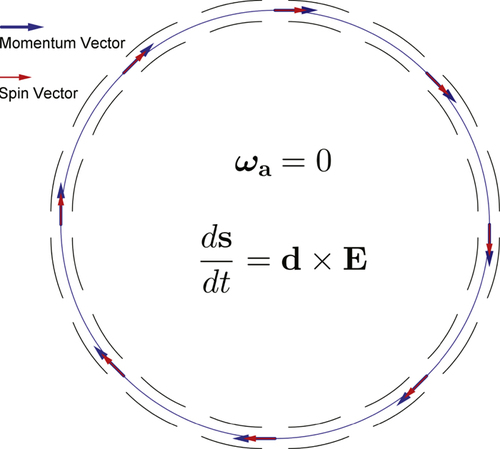
\includegraphics[width=.7\linewidth]{FS_ring}}; % из Proton EDM proposal
	\pause
	\node (real) at (scheme.center){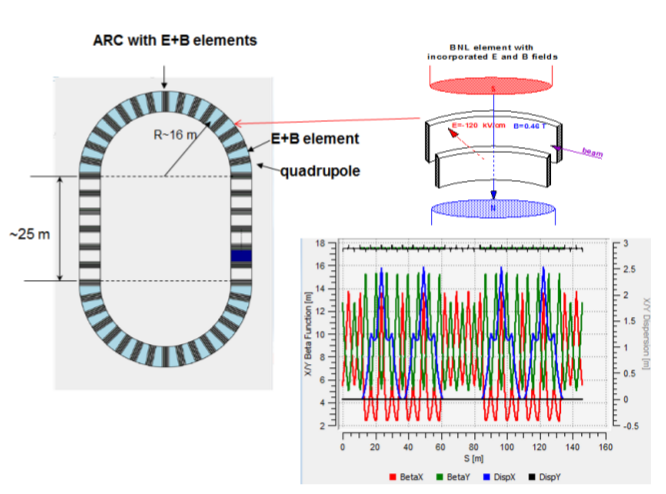
\includegraphics[width=.9\linewidth]{chapter2/BNL_lattice}};
\end{tikzpicture}
\end{frame}

%\begin{frame}{Варианты структур}
%\framesubtitle{Истинно-замороженный спин}
%\centering
%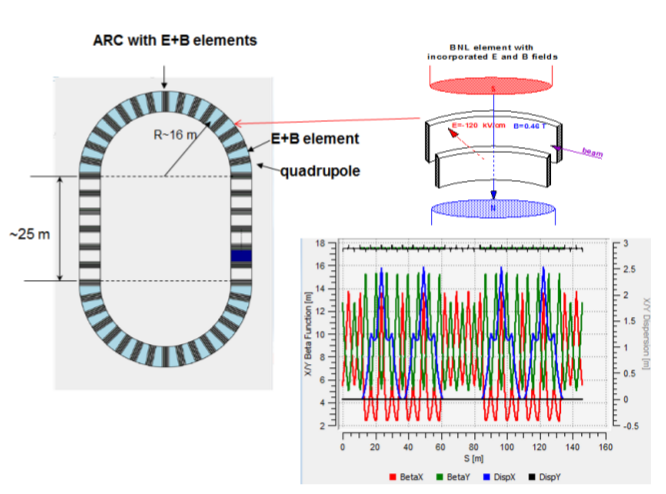
\includegraphics[width=.8\linewidth]{chapter2/BNL_lattice}
%\end{frame}
%
%\begin{frame}{Варианты структур}
%\framesubtitle{Квази-замороженный спин}
%\centering
%\begin{tikzpicture}
%\node (SX) {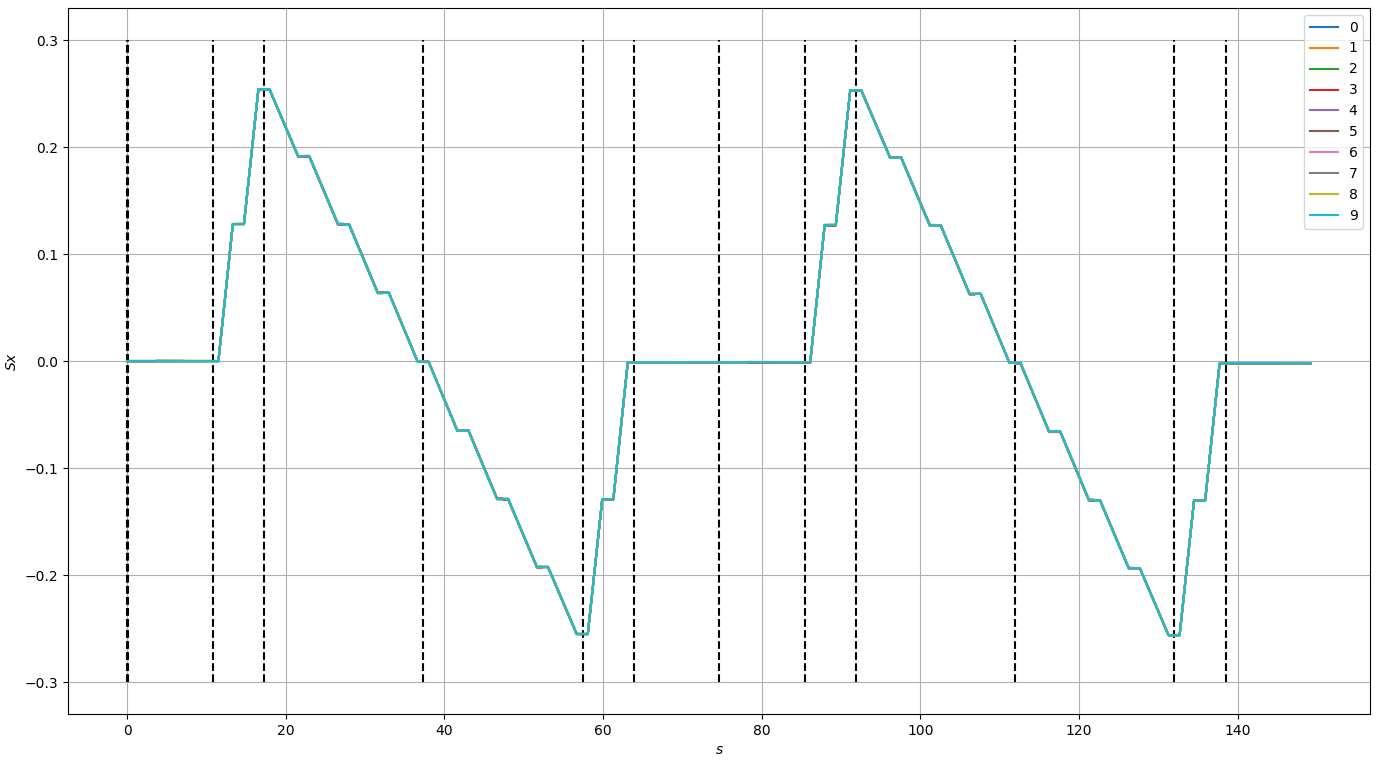
\includegraphics[width=\linewidth]{chapter2/EB_QFS_Sx_vs_s_1turn}};
%\pause
%\node (form) at (SX.north east) [xshift=-2cm, yshift=.5cm] {$J_0(\Phi_s) \approx 1 - \frac{\Phi_s^2}{4}$};
%\pause
%\node (6_3) at (SX.center)[xshift=-2cm, yshift=2cm]
%{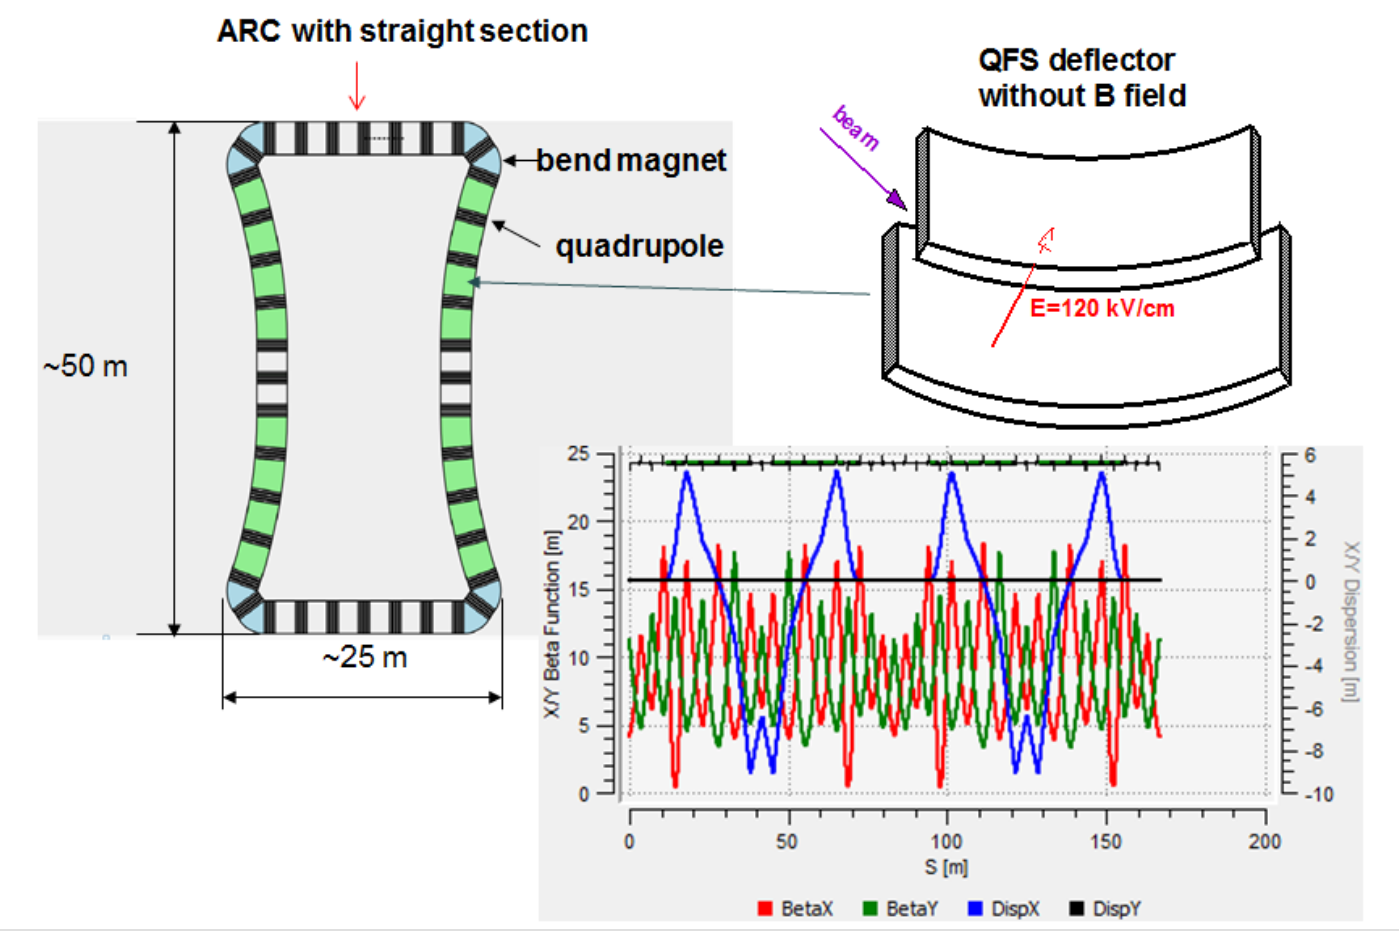
\includegraphics[width=.7\linewidth]{chapter2/6_3_lattice}};
%\pause
%\node (EB) at (SX.center)[xshift=2cm, yshift=-.07cm]
%{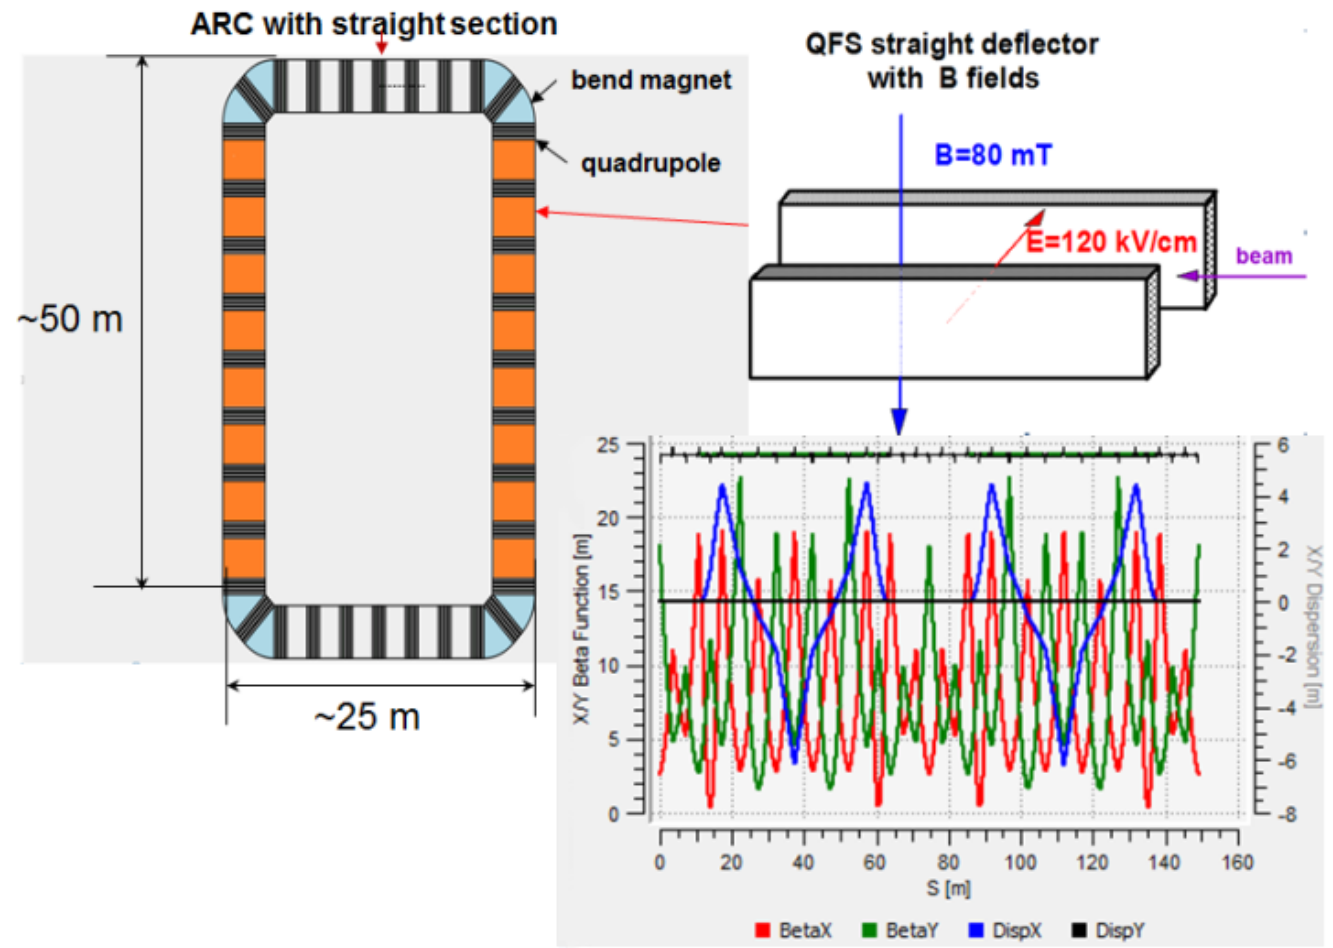
\includegraphics[width=.7\linewidth]{chapter2/E+B_lattice}};
%\end{tikzpicture}
%\end{frame}

%\begin{frame}{Измерение амплитуды vs частоты}
%\[
%P_y = A\cdot \sin\Big[\underbrace{\sqrt{(\w_{edm} + \w_{imp})^2 + \w_y^2 + \w_z^2}}_{\W}\cdot t + \delta\Big]
%\]
%\begin{itemize}
%	\item \textbf{Амплитуда:} 
%	\begin{itemize}
%		\item Останавливаем МДМ-прецессию и в \textbf{горизонтальной}, и в \textbf{вертикальной} плоскости
%		\item Наблюдаем за изменением \textbf{пространственной ориентации} вектора поляризации пучка
%	\end{itemize}
%	\item \textbf{Частота:}
%	\begin{itemize}
%		\item Останавливаем МДМ-прецессию \textbf{только} в горизонтальной плоскости
%		\item Наблюдаем за изменением в \textbf{угловой скорости} прецессии поляризации в вертикальной плоскости
%	\end{itemize}
%\end{itemize}
%\end{frame}
%
%\begin{frame}{Достоинства частотного метода}
%\begin{itemize}
%\item Менее жёсткие условия на точность установки элементов (не нужно исключать МДМ-вращение в вертикальной плоскости)
%\item Устойчивое состояние \textbf{двумерно}-замороженного спина (решает проблему геометрической фазы)
%\item Проще в отношении поляриметрии
%\end{itemize}
%\end{frame}

\section{Экспериментальная база}
%%%%%%%%%%%%%%%%%%%%%%%%%%%%%%%%%%%%%%%%%%%%%%%%%%%%%%%%%%%%%%%%%%%%%%%%%%%%%%%%%%%%%%%%%%%%%%%%%%%%%%%
\begin{frame}{Синхротрон COSY}
	\centering
	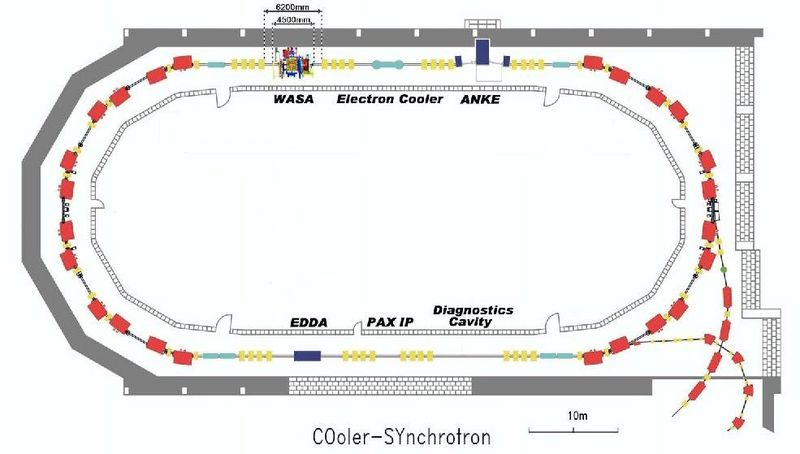
\includegraphics[width=.8\linewidth]{chapter4/800px-COSY_RING}
\end{frame}

\section{Метод исследования}
%%%%%%%%%%%%%%%%%%%%%%%%%%%%%%%%%%%%%%%%%%%%%%%%%%%%%%%%%%%%%%%%%%%%%%%%%%%%%%%%%%%%%%%%%%%%%%%%%%%%%%
\begin{frame}{Код COSY Infinity}
	% Здесь про то, как Кози вычисляет трансфер матрицы
	\begin{itemize}
		\item Разработка М. Берца и К. Макино (Michigan State University)
		\item Основан на дифференциальной алгебре; позволяет вычислять трансфер-матрицы элементов до (потенциально) любого порядка разложения ряда Тэйлора
		\item Трэкинговый код, учитывающий спиновую динамику
	\end{itemize}
\end{frame}
\begin{frame}{Спин-трэкинг в COSY Infinity} 
	%З десь про то, что строятся орбитальная и и спин трансфер-матрицы, и что Т-БМТ в
	% спин трансфер матрице
	\[
	\begin{cases}
	\vec{z}_n &= \mathcal{M}(\vec{z}_{n-1}), \\
	\vec{S}_n &= \hat A(\vec z_{n-1})\cdot \vec S_{n-1}
	\end{cases}
	\]
\end{frame}

\section{Результаты моделирования}
%%%%%%%%%%%%%%%%%%%%%%%%%%%%%%%%%%%%%%%%%%%%%%%%%%%%%%%%%%%%%%%%%%%%%%%%%%%%%%%%%%%%%%%%%%%%%%%%%%%%%%%%
\begin{frame}{Эффект бетатронных колебаний}
\begin{block}{ЭДМ-статистика}
	$\hat\w_{edm} = \frac12(\hat\w_x^+ + \hat\w_x^-)$, где $\w_x^\pm = \w_{edm} \pm \w_{mdm}$
\end{block}
%\pause
\begin{block}{Частота оценивается путём фитирования}
	$f(t) = a\cdot\sin(\omega_x\cdot t + \delta) \mapsto \hat\w_x$, где $(a,\omega, \delta) = \const$
\end{block}
%\pause
\begin{block}{Решение Т-БМТ уравнения даёт}
	$a = \sqrt{\nbar_x^2 + (\nbar_y\cdot\nbar_z)^2}$, где $\nbar = g(\vec E, \vec B)$
\end{block}
\end{frame}

\begin{frame}\centering
\begin{tikzpicture}
\node(NBAR) {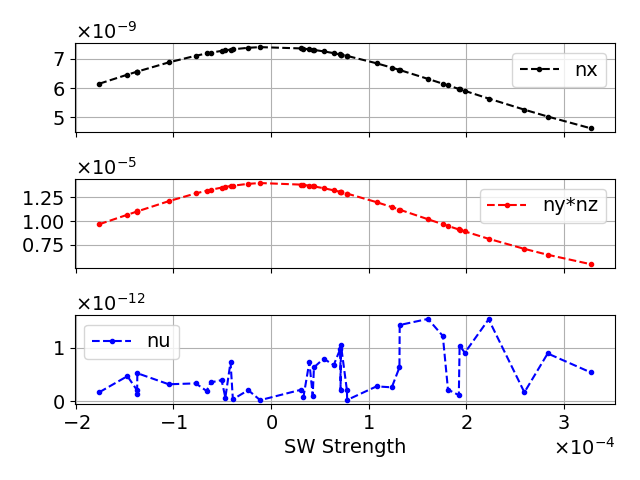
\includegraphics[width=.8\linewidth]{smp_sim/NBAR_variation_sd_vs_SW}};
\pause
\node (resid) at (NBAR.center)[xshift=2cm, yshift=-2cm] {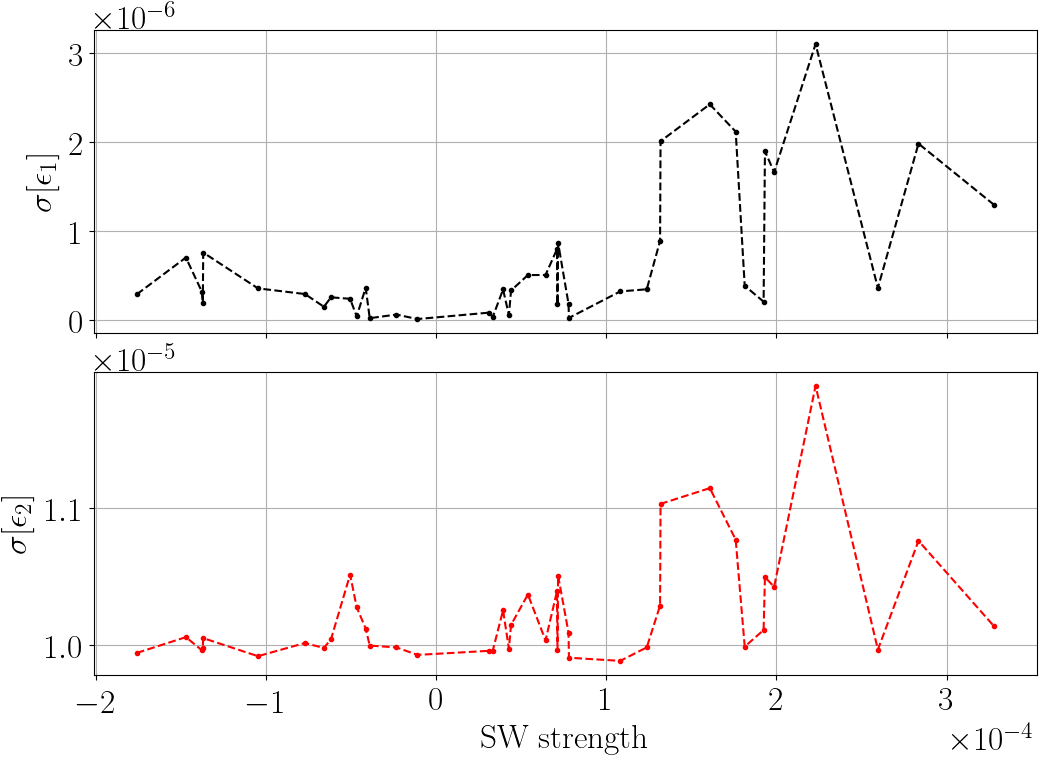
\includegraphics[width=.7\linewidth]{smp_sim/residual_SD_vs_SW(both)}};
\end{tikzpicture}
\end{frame}

\begin{frame}{Выводы}
\begin{enumerate}
\item Осцилляции амплитуды сигнала пренебрежимо малы
\item Коэффициент корреляции $\sigma[\hat a, \hat\w] < 10\%$
\item Эффект поддаётся контролю (при использовании частотного метода)
\end{enumerate}
\end{frame}



%\begin{frame}{Эффект неидеальности ускорителя}
%\centering
%\begin{tikzpicture}
%\node (null) {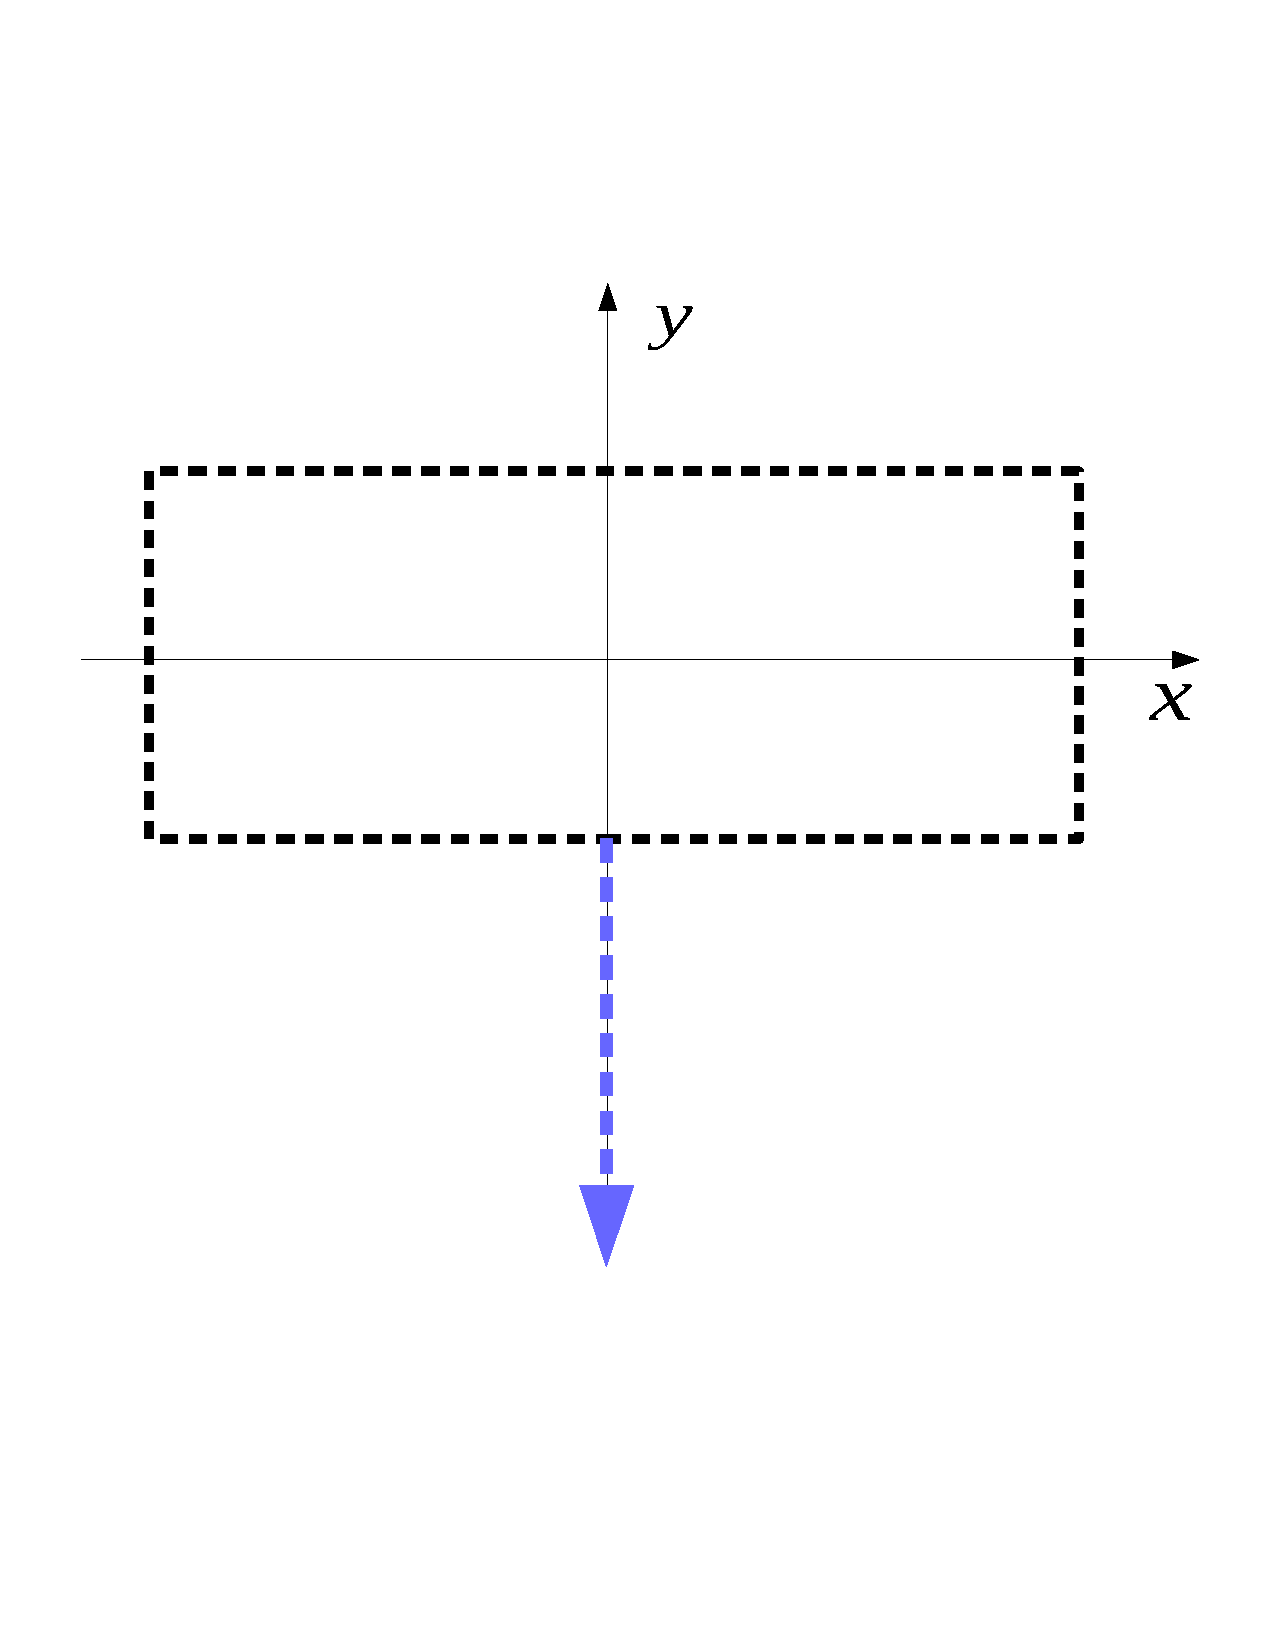
\includegraphics[height=.7\paperheight, trim=5 145 0 135, clip]{images/magnet_tilted-0.pdf}};
%\foreach \i in {1,...,3}
%{
%	\pause
%	\node (\i) at (null.center) {\includegraphics[height=.7\paperheight, trim=5 145 0 135, clip]{images/magnet_tilted-\i.pdf}};
%}
%\node (eq) at (null.south east)[yshift=.4cm] {$\hat\W_{edm} = \frac12\bkt{\W_x^{CW} + \W_x^{CCW}}$};
%\end{tikzpicture}
%\end{frame}

%\begin{frame}{Калибровка МДМ-сигнала}
%\begin{enumerate}[<+->]
%\item Подавляем спин-прецессию в вертикальной плоскости с помощью специального спин-ротатора (Вин-фильтра)
%\item Подстраиваем ведущее поле так, чтобы получить замороженный спин для данного пучка
%\item Выключаем спин-ротатор; мы восстановили $\Wmdm_x$
%\end{enumerate}
%\end{frame}

\begin{frame}{Калибровка МДМ-сигнала}
\framesubtitle{Результаты симуляции}
\centering
\begin{tikzpicture}
\node (A) {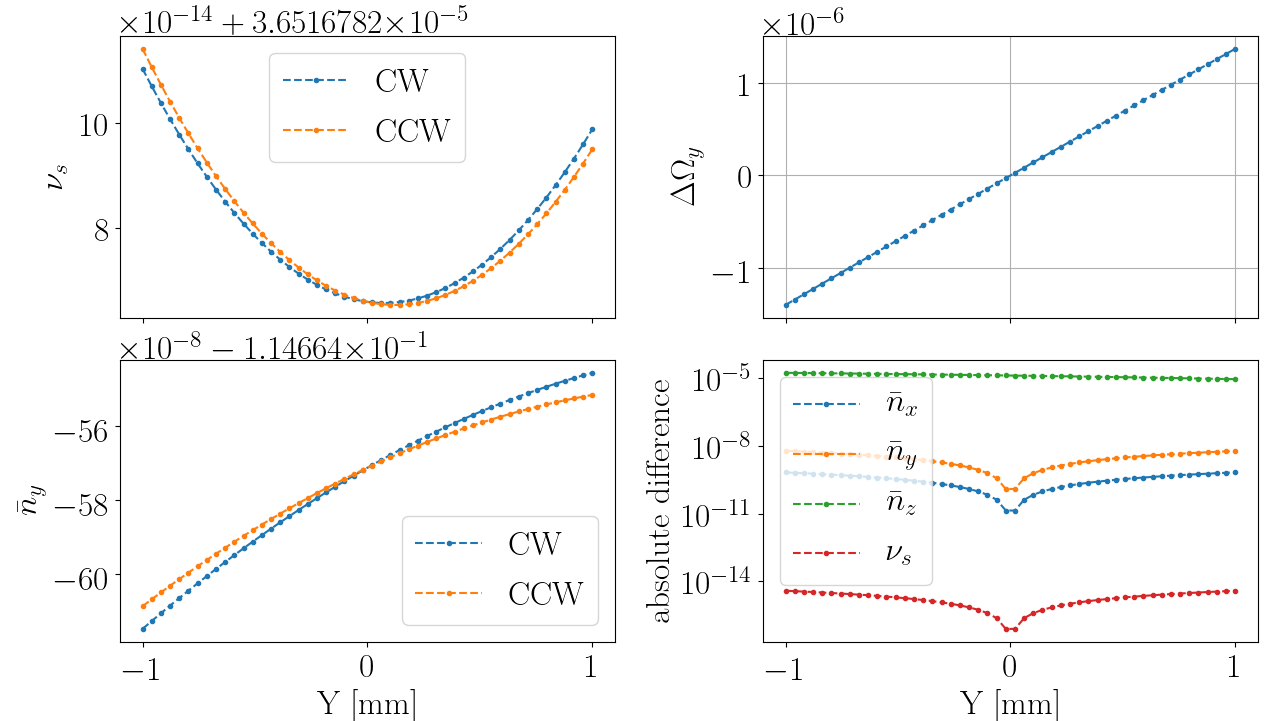
\includegraphics[width=\linewidth]{GFF/GFF_stune_range_Y}};
\pause
\node (B) at (A.center) {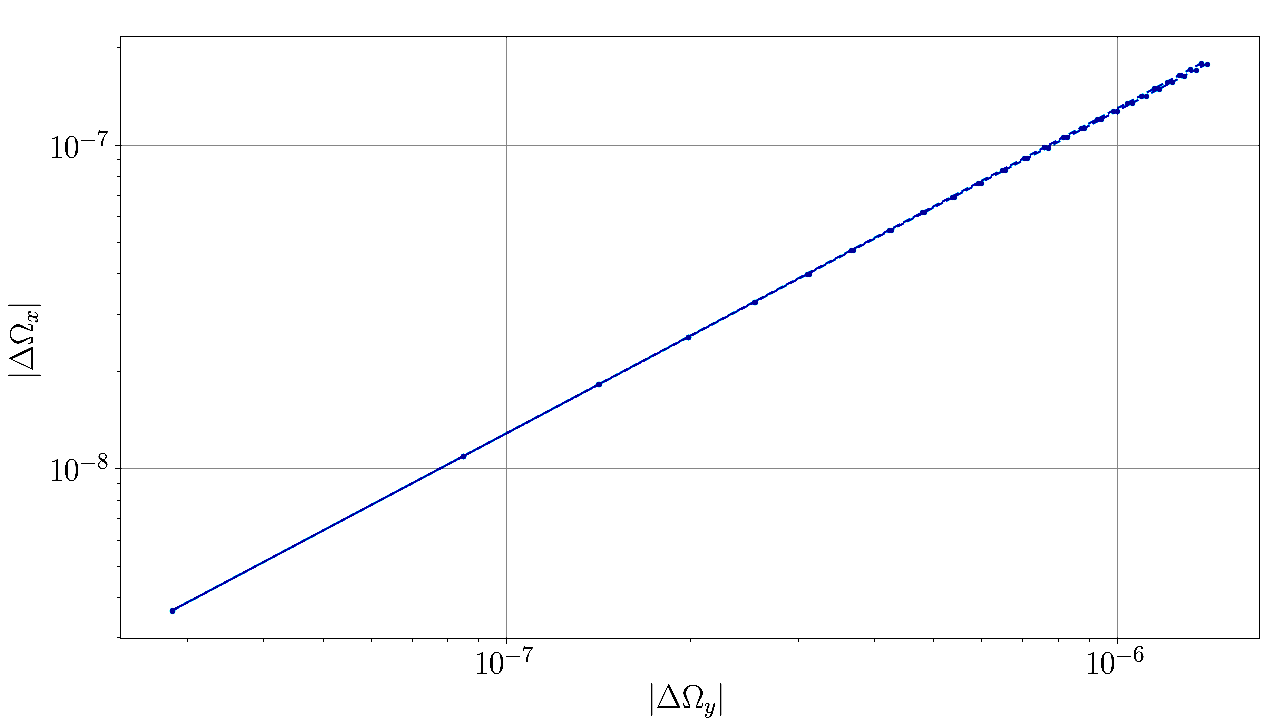
\includegraphics[width=\linewidth]{GFF/GFF_omegas_range_Y}};
\end{tikzpicture}
\end{frame}

\begin{frame}{Подавление спин-декогеренции}
\framesubtitle{Идеальная структура}
\centering
\begin{tikzpicture}
\node (X) {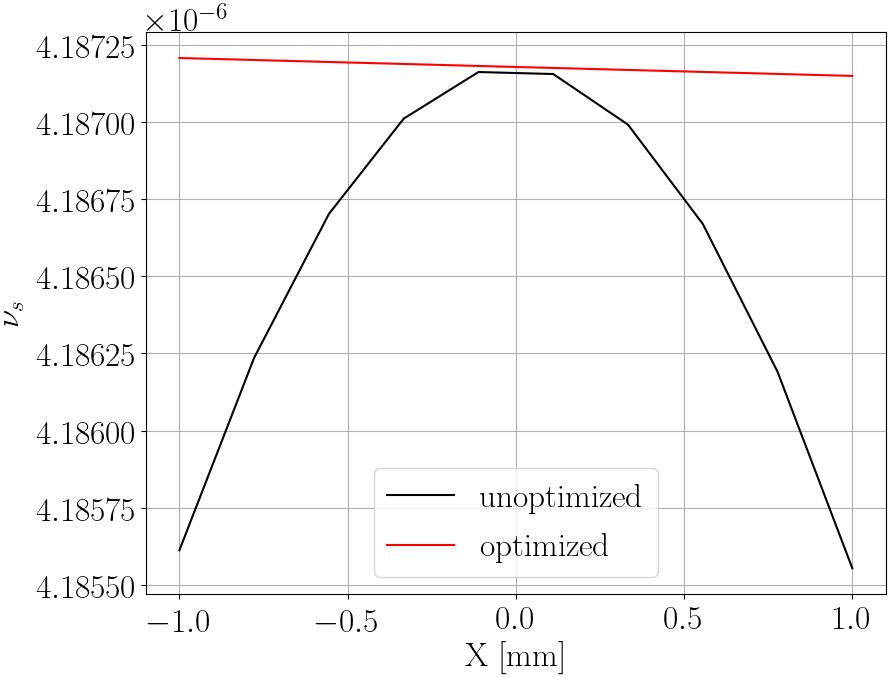
\includegraphics[height=.5\paperheight]{decoh_sim/spin_tune_decoh_x_offset}};
\pause
\node (Y) at (X.east)[yshift=-1.7cm]{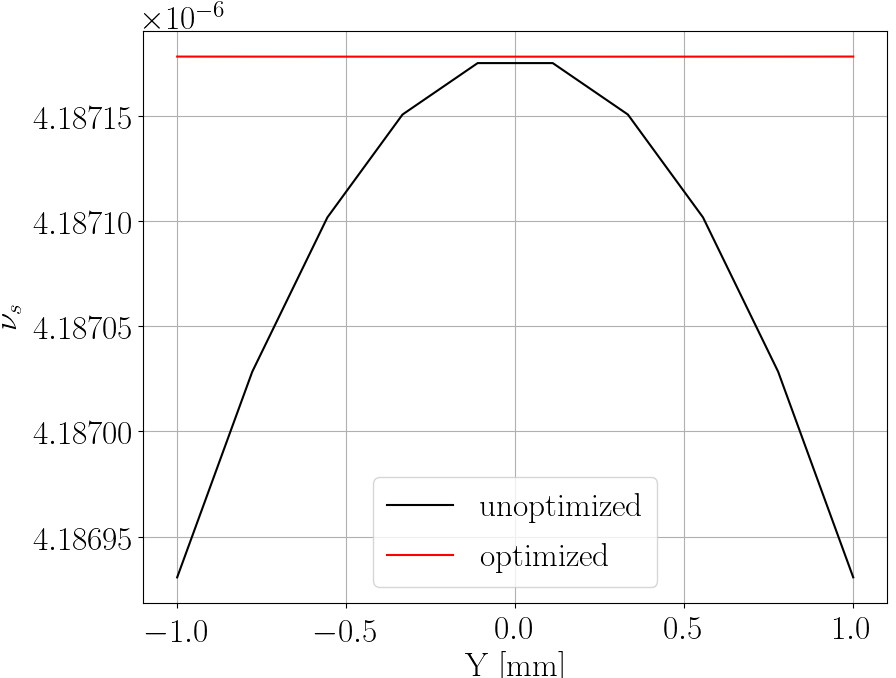
\includegraphics[height=.5\paperheight]{decoh_sim/spin_tune_decoh_y_offset}};
\pause
\node (D) at (X.center)[yshift=-2.3cm]{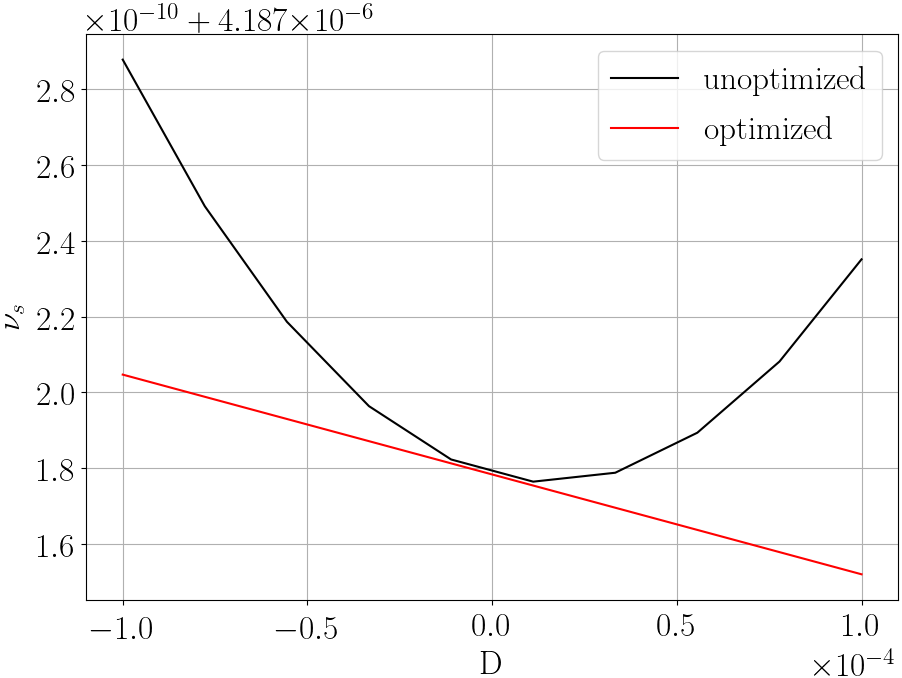
\includegraphics[height=.5\paperheight]{decoh_sim/spin_tune_decoh_d_offset}};
\end{tikzpicture}
\end{frame}
%\begin{frame}{Декогеренция в неидеальной структуре}
%\begin{tikzpicture}
%\node (imgX) {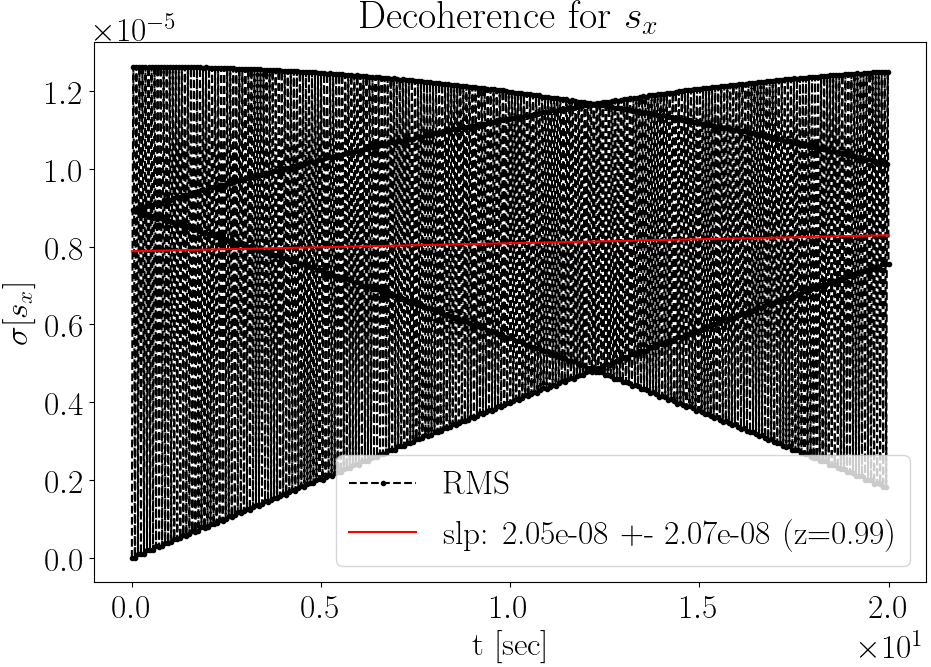
\includegraphics[width=.65\linewidth]{decoh_sim/SX_decoh_20sec_unopt}};
%\pause
%\node (imgY) at (imgX.south east)[yshift=1cm]{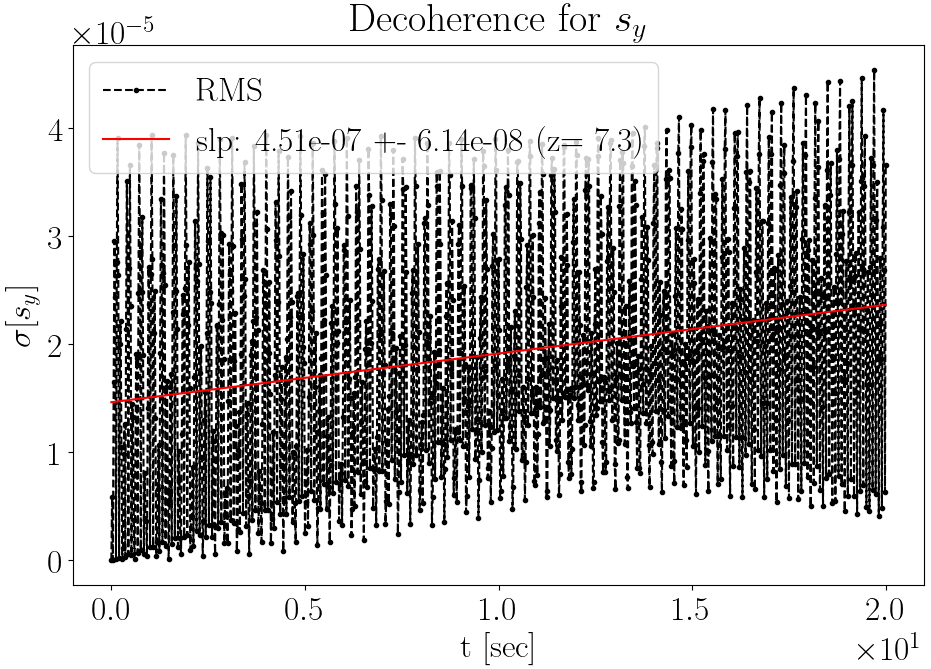
\includegraphics[width=.65\linewidth]{decoh_sim/SY_decoh_20sec_unopt}};
%\end{tikzpicture}
%\end{frame}
%\begin{frame}{Включаем секступоли}
%\begin{tikzpicture}
%\node (imgX) {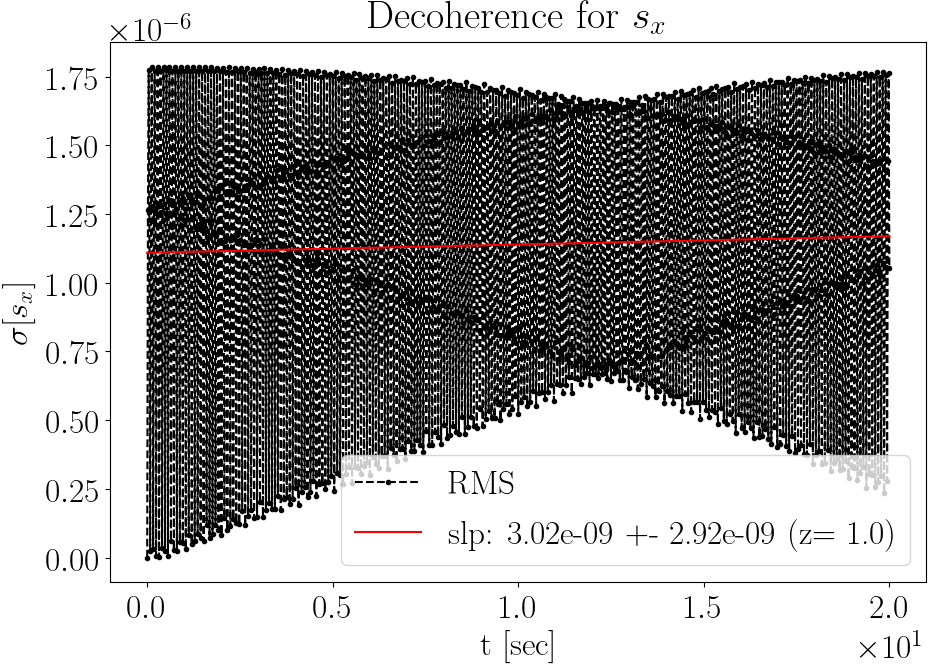
\includegraphics[width=.65\linewidth]{decoh_sim/SX_decoh_20sec_opt}};
%\pause
%\node (imgY) at (imgX.south east)[yshift=1cm]{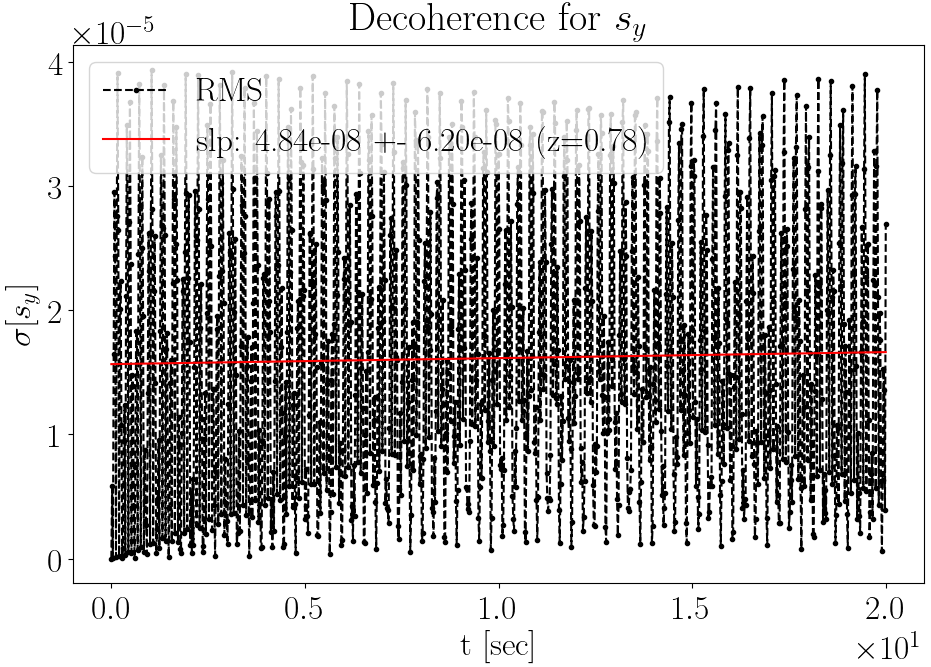
\includegraphics[width=.65\linewidth]{decoh_sim/SY_decoh_20sec_opt}};
%\end{tikzpicture}
%\end{frame}

\section{Результаты эксперимента}
%%%%%%%%%%%%%%%%%%%%%%%%%%%%%%%%%%%%%%%%%%%%%%%%%%%%%%%%%%%%%%%%%%%%%%%%%%%%%%%%%%%%%%%%%%%%%%%%%%%%%%%%
\begin{frame}{Исследования на COSY}
\framesubtitle{Спин-декогеренция}
\centering
\begin{tikzpicture}
\node (COSY) {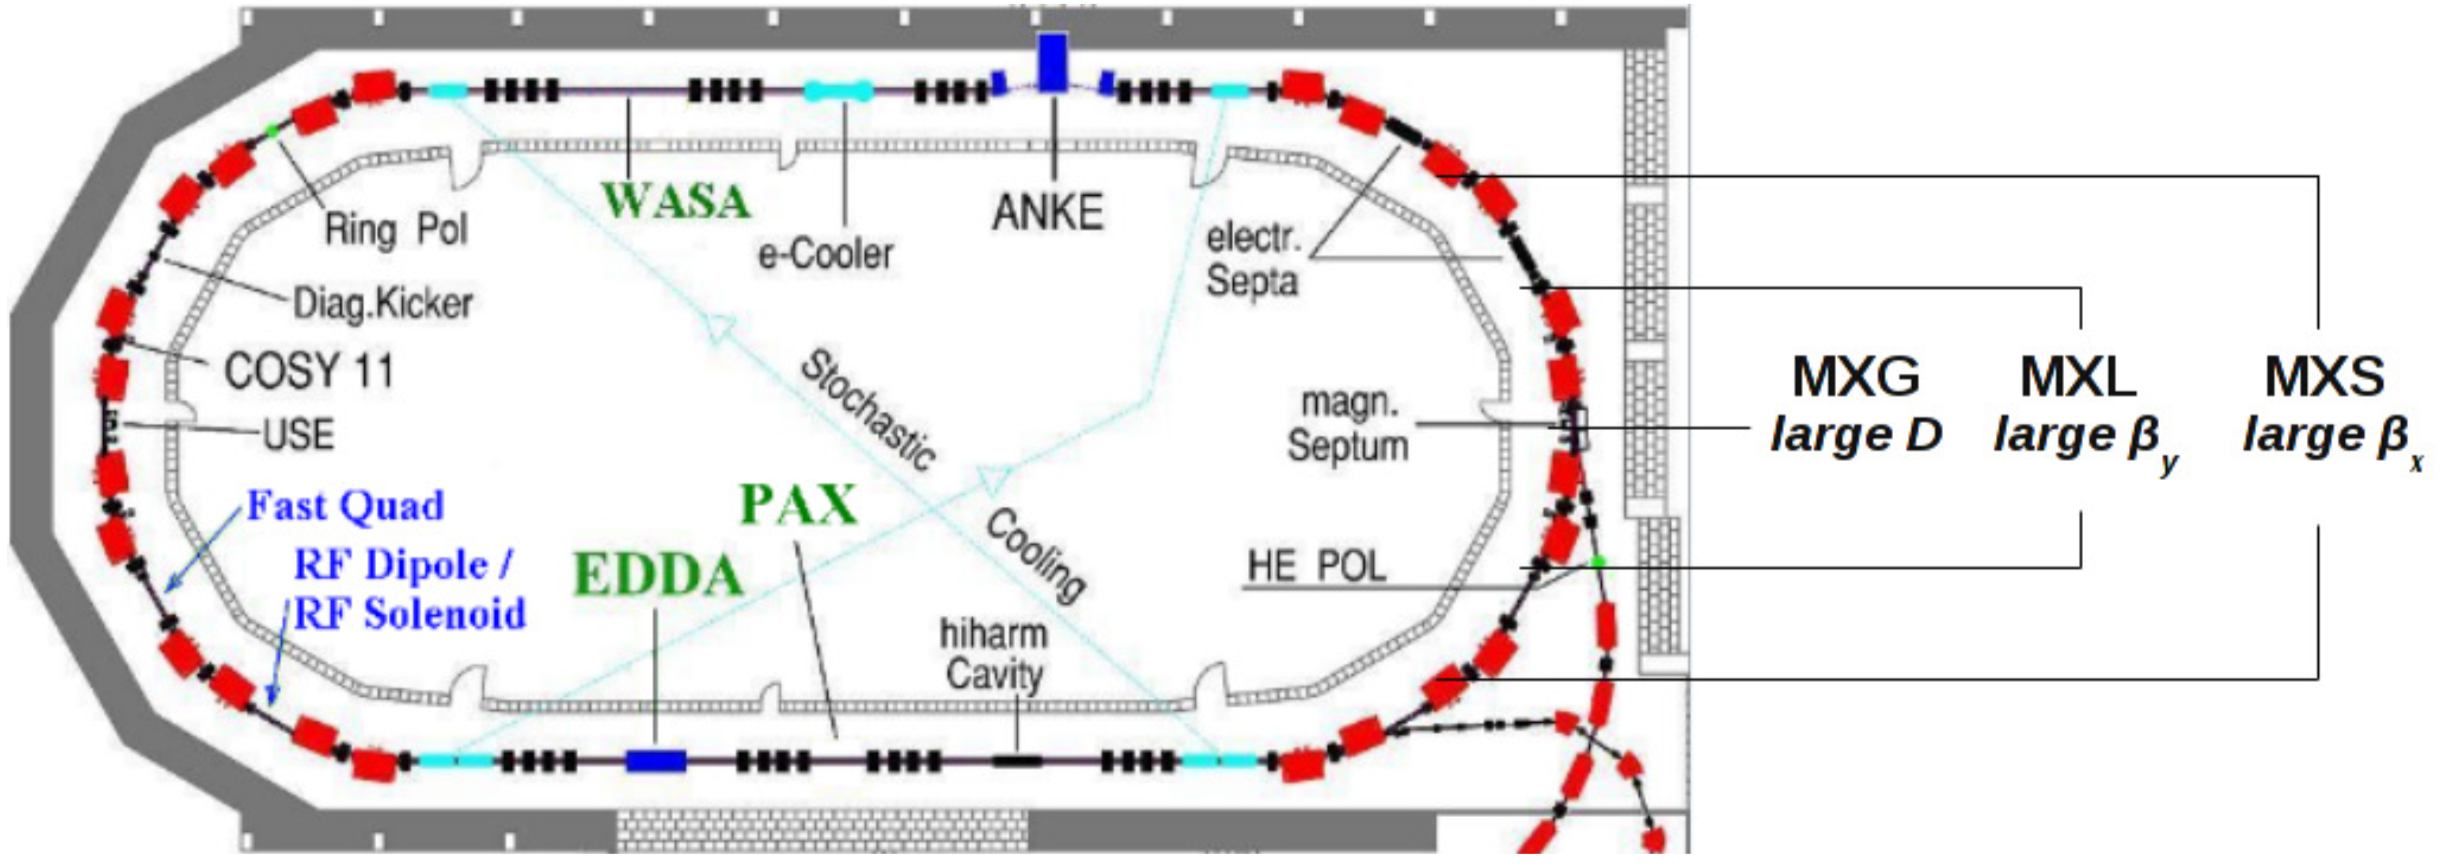
\includegraphics[width=.9\linewidth]{chapter4/COSY-sextupoles}};
\pause
\node (imgA) at (COSY.north east) [xshift=-3cm] {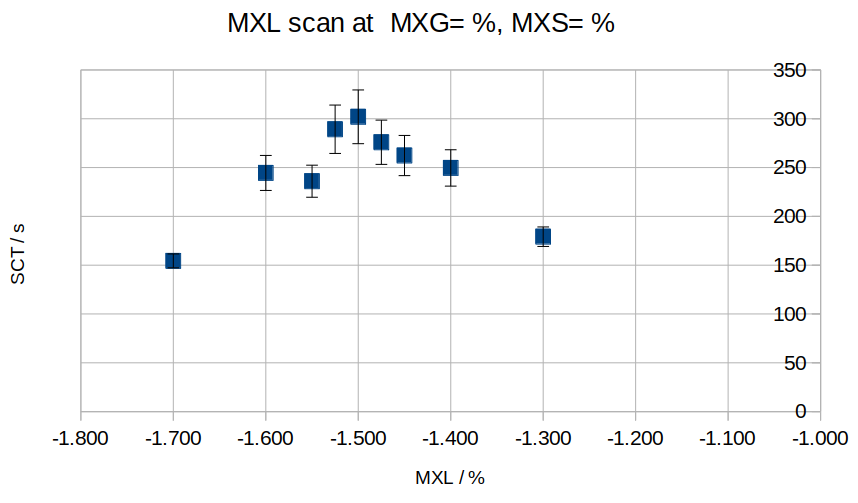
\includegraphics[width=.6\linewidth]{chapter4/SCT-April-2019/MXL_scan}};
\pause
\node (imgB) at (COSY.south west) [xshift=3cm, yshift=1cm] {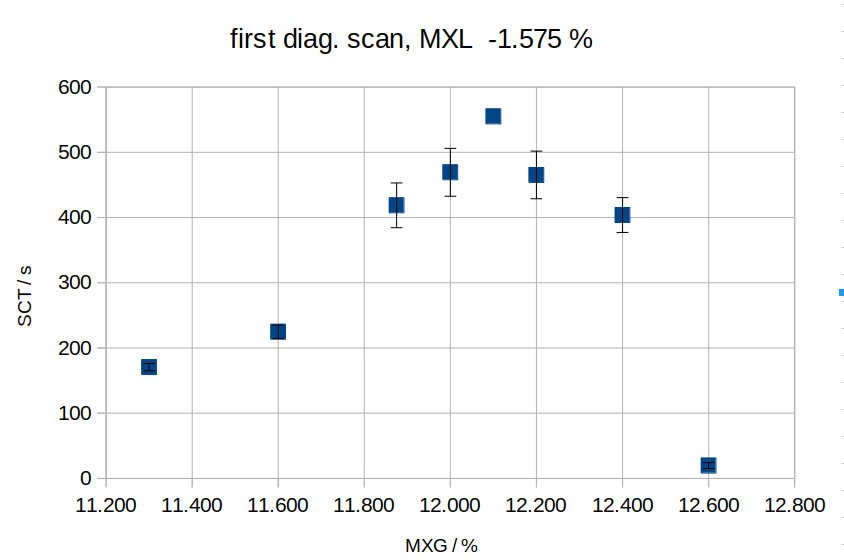
\includegraphics[width=.6\linewidth]{chapter4/SCT-April-2019/MXG_scan}};
\end{tikzpicture}
f\end{frame}

\section{Формальные вещи}


\begin{frame}{Результаты работы}
	\begin{enumerate}
		\item Изучены эффекты спиновой динамики вблизи нулевого спинового резонанса
		\item Описаны и численно промоделированы средства борьбы с этими эффектами
		\item Сформулирован аргумент в пользу частотного метода измерений ЭДМ в накопительном кольце с замороженным спином
	\end{enumerate}
\end{frame}

\begin{frame}{Положения выносимые на защиту}
\begin{itemize}
	\item ЭДМ-статистика частотного метода измерения не чувствительна к возмущениям со стороны бетатронного движения частиц
	\item Возможно достичь времени жизни поляризации пучка на уровне 1000 секунд
	\item Свойства угловой скорости МДМ-прецессии 
	\begin{itemize}
		\item вынуждают использование частотных методов измерения ЭДМ
		\item оставляют возможность исключения этой систематической ошибки из конечной статистики
	\end{itemize}
\end{itemize}
\end{frame}
\begin{frame}
\begin{itemize}
\item Зависимость частоты прецессии спина частицы может быть выражена как функция одной переменной, называемой эффективным Лорнец-фактором, и отражающей величину продольного эмиттанса частицы
\item Эффективный Лоренц-фактор поддаётся калибровке
\item Возможно достичь величины стандартной ошибки среднего значения ЭДМ-статистики на уровне $10^{-29}$\ecm~за год измерений
\end{itemize}
\end{frame}

%\begin{frame}
%\begin{center}
%Спасибо за внимание!
%\end{center}
%\end{frame}

%\begin{frame}[allowframebreaks]
%	\frametitle{Основные публикации по теме диссертации}
%	\begin{thebibliography}{9}
%		\bibitem{Stats-LaPlas}
%		A.E. Aksentev, Y.V. Senichev, ``Statistical precision in charged particle {EDM} search in storage rings.'' J. Phys.: Conf. Ser. \textbf{941} 012083 (2017)
%		\bibitem{Stats-IPAC}
%		A.E. Aksentyev, Y.V. Senichev,
%		``Model of Statistical Errors in the Search for the Deuteron EDM in the Storage Ring,''
%		in \emph{Proc. IPAC'17}, Copenhagen, Denmark, May 2017, pp. 2258--2260,
%		\url{https://doi.org/10.18429/JACoW-IPAC2017-TUPVA079}.
%		\bibitem{SOD-modeling-LaPlas}
%		A. Aksentev ``Modeling of spin-orbital dynamics in a storage ring.'' J. Phys.: Conf. Ser. \textbf{1238} 012079 (2019)		
%		\bibitem{SD-LaPlas}
%		A. E. Aksentyev, Y. V. Senichev, ``Spin Decoherence in a Frozen Spin Lattice, Its Suppression and Effect on the Frequency Domain Edm Statistic,''  в процессе публикации.
%		\bibitem{GFF-IPAC}
%		A.E. Aksentyev, Y.V. Senichev, ``Simulation of the Guide Field Flipping Procedure for the Frequency Domain Method,'' in \emph{Proc. IPAC'19}, Melbourne, Australia, May 2019, pp. 858--860, \url{doi:10.18429/JACoW-IPAC2019-MOPTS010}
%		\bibitem{SMP-IPAC}
%		A.E. Aksentyev, Y.V. Senichev, ``Spin Motion Perturbation Effect on the EDM Statistic in the Frequency Domain Method,'' in \emph{Proc. IPAC'19}, Melbourne, Australia, May 2019, pp. 861--863,
%		\url{doi:10.18429/JACoW-IPAC2019-MOPTS011}
%		\bibitem{SD-IPAC}
%		A.E. Aksentyev, Y.V. Senichev, ``Spin Decoherence in the Frozen Spin Storage Ring Method of Search for a Particle EDM,'' in \emph{Proc. IPAC'19}, Melbourne, Australia, May 2019, pp. 864--866,
%		\url{doi:10.18429/JACoW-IPAC2019-MOPTS012}
%	\end{thebibliography}
%\end{frame}

\end{document} 
